% # -*- coding: utf-8 -*-
\section{Introduction}\label{seciton:introduction}
% オペレーティングシステム(OS)カーネルに対する攻撃として,特権昇格攻撃とセキュ
% リティ機能の無効化攻撃が課題とされている.
%
The operating system (OS) kernel encounters threats, in which privileges may be
escalated and security mechanisms may be defeated.
% defeat of security mechanism.
% attacks are considered 
% %
% これらの攻撃は,攻撃者のユーザプロセスが,脆弱性を含むカーネルコード(以降,
% カーネル脆弱性)を利用し,メモリ破壊を起こし,権限情報の改ざん,ならびにセキュ
% リティ機能の回避のためにセキュリティ機能に関するカーネルデータを改ざんする攻撃
% である.
% These attacks are attacks in which 
The user process of the adversary exploits the kernel code containing
vulnerabilities (i.e., vulnerable kernel code), thereby corrupting the memory.
%resulting in memory corruption.
%
The kernel vulnerability is reported by the Common Vulnerabilities and Exposures
(CVE) \cite{cve}. The CVE has the Common Platform Enumeration (CPE) that indicates the naming of
systems, software, and packages \cite{cpe}.
%
Until August 2022, 724 CVE with CPE of Linux (e.g., \verb|linux_kernel|) and CVE
description contains specific word (e.g., ``memory'') were issued in the CVE of
National Vulnerability Database (NVD) \cite{nvd}, as shown in
\figref{fig:linux_memory_cve}.

\begin{figure}[tb]
  % \begin{center}
    % \hspace*{-25.0ex}
    % \begin{tabular}{cc}
    % \begin{minipage}[t]{0.80\hsize}      
      %\begin{figure}[t]
    %  \vspace{-15ex}  
    \hspace{-5ex}
        \begin{center}
          \includegraphics[bb=0 0 464 296, scale=.500]{./imgs/X001_linux_cve_memory_stats.png}
        \end{center}
  %\includegraphics[bb=0 0 645 986, scale=.240]{./imgs/A01X_05_screenshot_2021-06-04_17_29_08.png}  
  %\includegraphics[scale=.260]{./imgs/05_screenshot_2021-06-04_17_29_08.eps}
    %  \vspace{-4.5ex}  
    % \vspace{-1.0ex}    
        \caption{
          %
          Statistics of CVE for Linux kernel memory until August 2022 \cite{nvd}
          %
        }
        \label{fig:linux_memory_cve}
%\vspace{-5.0ex}        
\end{figure}

% It achieves the illegal modification of privileged information and alters kernel
% data of the security mechanism to take full administrator privileges.
%
Therefore, privileged information can be modified and kernel data of the security
mechanism can be altered to gain full administrator privileges.
%  bypass security functions.
% %
% 攻撃事例として,特権奪取攻撃に加え,セキュリティ機能の無効化攻撃ではアクセス
% 制御特権昇格攻撃に加え,セキュリティ機能の無効化攻撃の事例では,
%
% 攻撃事例として,アクセス制御に関するカーネルデータを改ざんの後,管理者権限に昇
% 格し,制限の回避が試みられる\cite{nexus5exploit,grsecurity}.
% From and actual attack case, 
The actual kernel memory corruption cases indicate that the modifying the kernel data
related to mandatory access control (MAC), the user acquires administrator
privileges and circumvents the MAC restrictions \cite{nexus5exploit,grsecurity}.

% オペレーティングシステム(OS)カーネルへの攻撃として,権限情報を管理者
% に改ざんする特権奪取攻撃が課題とされている.
% 特権奪取攻撃は,攻撃を行うユーザプロセスが脆弱性を含むカーネルコード
% (以降,カーネル脆弱性)を利用し,カーネル仮想記憶空間上に配置され,権
% 限情報を格納したカーネルデータに対し,一般ユーザから管理者ユーザ
% に改ざんする攻撃である.
% %
% 攻撃を行うユーザプロセスは計算機の管理者ユーザとして,マルウェアの実行
% や隠蔽を行い,他の計算機への攻撃を試みる.

%
% An operating system (OS) kernel must have the ability to tackle
% vulnerable kernel codes, which can otherwise lead to memory corruption
% or denial of service (DoS), among other problems.
% %
% Moreover, such attacks can leverage privilege escalation or service
% disruption to cause further damage, or suspend the running kernel altogether
% \cite{chen11linux}.

% カーネル脆弱性を介した攻撃の防止手法として,Kernel Address Space Layout
% Randomization (KASLR)は,カーネルコードやカーネルデータの仮想アドレスをランダ
% ム化し,攻撃時の仮想アドレスの特定を困難化した \cite{shacham04ccs}.
% %
% また,不正コード呼出し制限のため,KCoFIでは,コード呼出し順を検査するControl
% Flow Integrity(CFI)\cite{abadi05ccs}をカーネルに適用可能とした
% \cite{criswell14sp}.

% カーネル脆弱性を利用した攻撃の防止手法として,KCoFIでは,コード呼出し
% 順を検査する control flow integrity(CFI)\cite{abadi05ccs}をカーネル
% に適用可能とし,不正なコード呼出しを制限した \cite{criswell14sp}.
% As a method to prevent attacks using kernel vulnerabilities, KCoFI enables
The following are the countermeasures that can prevent kernel attacks via
vulnerable kernel code. Kernel control flow integrity (KCoFI)
% enables control flow integrity (CFI) 
inspects the order of code execution \cite{abadi05ccs} to restrict the
kernel code from being illegally invoked \cite{criswell14sp}.
% Kernel address space layout randomization (KASLR)では,カーネルの仮
% 想記憶空間上のカーネルコードやカーネルデータの仮想アドレスをランダム化
% し,攻撃時の仮想アドレスの特定を困難化した \cite{shacham04ccs}.
Kernel address space layout randomization (KASLR) randomizes the virtual
addresses of the kernel code and kernel data in the kernel memory space to foil
attacks \cite{shacham04ccs}, whereas
% This makes it difficult to identify the virtual address during an attack
%
% また,特権奪取攻撃対策として,Additional kernel observer(AKO)は,カーネルに
% おける権限情報変化に対し,意図しない書替えを検知した場合,元の権限情報に修正
% し,特権奪取攻撃の防止を実現している \cite{yamauchi21ijis}.
%In addition, 
the additional kernel observer (AKO) detects unintentional rewriting in response
to the changes in the privileged information of user processes against a privilege
escalation attack \cite{yamauchi21ijis}.
% the original privilege information
% when it This prevents privilege-grabbing attacks
% \cite{yamauchi21ijis}.

% 既存の手法により,カーネルにおける,カーネル脆弱性を介したカーネルデータ改ざん,
% ならびに不正コード呼出しは軽減される.しかし,攻撃が成功した場合,権限情報やセ
% キュリティ機能に関するカーネルデータは改ざん可能であり,以下の課題があると考えて
% いる.
% 既存の手法では,ユーザプロセスからの特権奪取攻撃の成立困難化として,脆
% 弱なカーネルコード特定,呼出し,ならびに被害の抑制を行う.しかし,権限
% 情報に対する攻撃自体は可能であり,次の課題があると考えている.
% Existing techniques 
%These mitigate illegal modifications of kernel data via kernel vulnerabilities.
These mitigate the kernel data from being illegally modified via kernel
vulnerabilities.
% and malicious code calls in the kernel. 
However, if the kernel memory is successfully corrupted, kernel data can be
overwritten.
%authorization information and security functions 
%
%
% Kernel hardening approaches adopt software and hardware based
% mechanisms. Kernel control flow integrity \cite{abadi05ccs}, kernel
% address randomization (KASLR) \cite{shacham04ccs}, and kernel isolation
% \cite{proclocal,sci} are mechanisms used to harden kernel codes and data
% against attacks.
% %
% A central processing unit (CPU) privilege mechanism provides access and
% execution restrictions between the user and the kernel mode \cite{smap-smep}.
% %
% However, the running kernel still contains vulnerable kernel codes,
% which can be invoked from an adversary's user process.
% \begin{enumerate}[topsep=0pt, leftmargin=1.2cm]%\itemsep=-1.0ex \parskip=1.0ex
%   \item [課題]: {\bf メモリ破壊によるカーネルデータの改ざん}\\
%     %
%     動作中のカーネルは,カーネルモードにおいて,カーネルデータの書込み制限は行わない.カーネル脆弱性
%     を利用し,メモリ破壊に成功する場合,攻撃者は権限情報やセキュリティ機能に関する
%     カーネルデータを書替え可能である.
%     %
%     従来手法では,セキュリティ機能に関するカーネルデータの書込み制限の制御は行われ
%     ないことから,改ざん防止は困難である.
% 特権奪取攻撃では,権限情報の改ざんとして,一般ユーザから管理者ユーザ
% へのユーザIDの書替えが行われる.
% %
% 従来手法では,権限情報は動作中のカーネルに対して読書き制限の制御は行
% われない.
% %カーネルモードにおいては読書き権限の制御は行われていない.
% %
% 実行されたカーネルコードには権限情報の書替え制限は行われないことから,
% 攻撃を行うユーザプロセスから脆弱なカーネルコードを実行された場合,権
% 限情報の改ざんを防ぐことは難しい.
% We consider the following issue induces 
We consider that a running kernel does not restrict the writing of kernel data
in the kernel mode. 
% If the kernel vulnerability is exploited and memory corruption succeeds,
% an adversary can rewrite kernel data. 
% related to authorization information and security functions.
%
Existing approaches do not control the write restrictions of kernel data related to
privileged information and security mechanisms. Therefore, an adversary can 
gain full administrator privileges.
% still take 
% , making it difficult to preventtampering.
%
%     %
% \end{enumerate}
% The identification and restraint of vulnerable kernel code in a running
% kernel is challenging. 
% %
% Although the common vulnerabilities and exposures (CVE) summarizes the overviews
% of kernel vulnerability, these report does not contain the detail of vulnerable
% kernel codes.
% %
% As modern kernels are complex and lengthy, it is hard to identify which kernel
% codes relate to which kernel vulnerabilities.
% %
% In addition, the removal of kernel codes can affect the stability of a user
% process or kernel.

% %
% Approaches, such as KASR and kRazor can reduce the kernel attack surface
% of a running kernel by restraining the vulnerable kernel code \cite{kurmus14dimva,
% zhang18arxiv}.
% %
% These approaches trace benign applications, related kernel codes, and kernel data to
% statically create available kernel images. It is necessary to regularly
% update the software to account for all applications and kernel-related behavior.
% %
% However, the past approaches do not target proof-of-concept (PoC) codes, which are
% small malicious program codes that target the invocation of vulnerable kernel codes
% to attack the kernel.

% 本稿では,特権奪取攻撃における,権限情報の改ざんを緩和するため,特定のカーネル
% データを保護対象(以降,保護対象カーネルデータ)として,書込み制限を動的に制御
% するセキュリティ機構を提案する.
In this study, we propose a kernel data protection mechanism (KDPM), which is
a novel security capability that dynamically controls the write restrictions of
specific kernel data as protected kernel data. 
% (hereinafter referred to as "protected kernel data").
% %
% \figref{fig:approach_overview}に提案手法の概要を示す.提案するセキュリティ機構
% では攻撃の種別に応じ,実現方式1,および実現方式2を備える.実現方式1では,汎用
% 性を重視し,特権昇格攻撃を防止する権限情報保護機能を実現している.実現方式1で
% は,ユーザプロセスに対し,予め許可されたシステムコール発行時のみに保護対象カー
% ネルデータへの書込みを許可する.
Figure \ref{fig:approach_overview} provides an overview of the KDPM,
%  is shown in Figure
%
% The proposed security mechanism 
which determines whether system calls and kernel codes have write permission of
the kernel data in the kernel layer.
%
To ensure kernel data protection and managing write restrictions, the KDPM
adopts the Intel memory protection key (MPK), which is a protection keys for
supervisor (PKS).
%
A PKS provides a protection key that handles write restrictions for each page of
kernel data.
% is specified for the kernel

%When a vulnerable kernel code is executed by the user process of an adversary,
%
The KDPM assumes that the user process of an adversary invokes a vulnerable
kernel code which attempts to modify the kernel data related to privileged
information or security mechanism.
%
The KDPM focuses the mitigation of the illegal overwritten of these kernel
data.
%as protected kernel data.}
% through the kernel memory corruption vulnerability. 
%
The privileged information is changed by specific system calls and the policy of
MAC is modified by specific kernel codes. Moreover, the function pointers of the MAC
are never modified at the running kernel.
%
%\cyanuline{ 
The KDPM provides a straightforward application of the PKS to maintain simple
design of the kernel data protection. Additionally, the KDPM combines the
characteristics of system calls, kernel code behavior, and hardware features. 
%}
%
The limitation of the KDPM is a little difficult to support frequently modified kernel data. 


\begin{figure}[tb]
  \centering        
  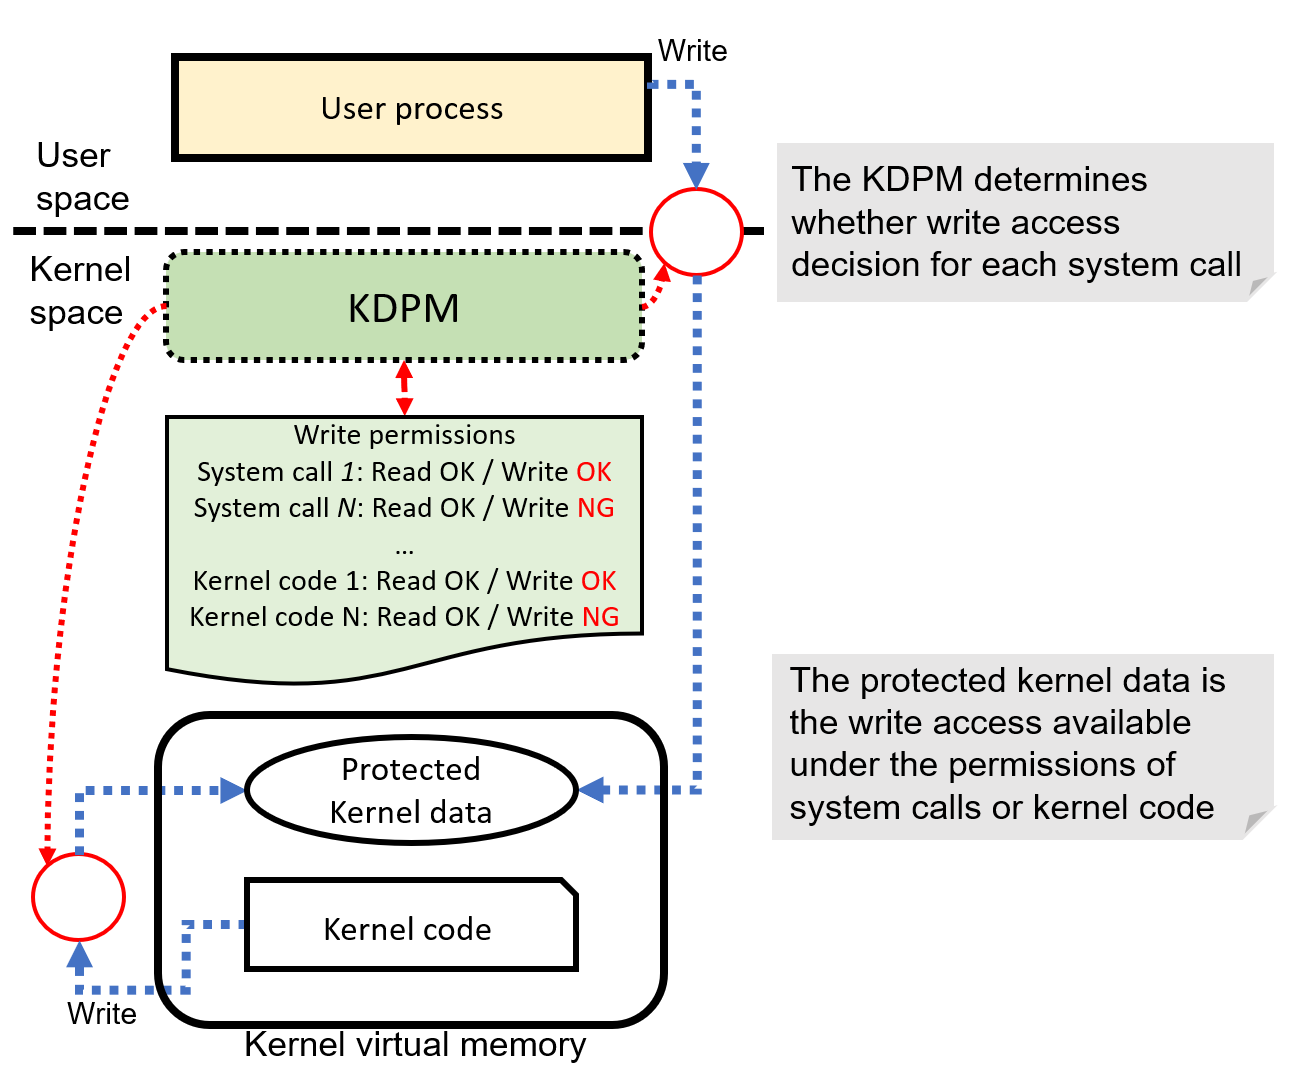
\includegraphics[bb=0 0 972 809, scale=.240]{./imgs/001_screenshot_2021-07-26_17.18.08.png}
  % \vspace{-2.0ex}  
  \caption{
    %
    %提案するセキュリティ機構の概要
    Overview of the kernel data protection mechanism
    %
  }
  \label{fig:approach_overview}
  %\vspace{-5.0ex}
  % \vspace{-2.0ex}  
\end{figure}


% Because the kernel allows the changing of privileged information using specific
% system calls. Additionally, the kernel has never modified the function pointer
% of MAC, and rarely changes MAC policy using specific kernel codes.}
% the privileged information or kernel data of security mechanism 

% the kernel memory corruption vulnerability
% that leads illegal overwritten of these kernel data. 
% that requires the memory write operation
% will not succeed unless the kernel disables the write restriction based on the
% PKS protection key.
% \red{The KDPM prevents the illegal overwritten of these kernel data through the
% kernel memory corruption vulnerability that requires the memory write operation
% will not succeed unless the kernel disables the write restriction based on the
% PKS protection key.}

The KDPM has two implementations that focus on the different types of kernel
attacks.
% i 1 and Realization 2, depending on the type of attack.
%
Implementation 1 is a general purpose for the protection of privileged
information to prevent privilege escalation. This allows user processes to write
to protected kernel data only when write-permitted system calls are invoked.
%
% 実現方式2として,カーネルデータの書き込み制限対象領域の細粒度化とオーバヘッド
% 低減を可能とする,セキュリティ機能の無効化攻撃を防止のためのセキュリティ機能保
% 護機能を検討する.実現方式1では,カーネルに対し,予め許可されたカーネルデータ
% の実行時のみに保護対象カーネルデータへの書込みを許可する.
Implementation 2 protects the kernel data of the security mechanism (e.g., MAC)
%protection function
to prevent security mechanism from being defeated. This reduces overheads to
limit the write restriction timing of protected kernel data.
%granularity and
Further, Implementation 2 allows the protected kernel data to be written only
when executing a write-permitted kernel code.

\begin{itemize}%[topsep=0pt]%\topsep=-1.0ex \itemsep=-1.0ex \parskip=1.0ex
%   \item {\bf 実現方式1}:特権昇格攻撃の防止のため,ユーザプロセスの権限情報の保護を目
%   的とし,システムコール単位にて権限情報の書込み制限を制御する手法
%   \item {\bf 実現方式2}:セキュリティ機能の無効化攻撃の防止のため,カーネルコード単位
%   にてセキュリティ機能に関するカーネルデータの書込み制限を制御する手法  


\item {\bf Implementation 1}: To prevent a privilege escalation attack,
Implementation 1 controls the write restriction of privileged information in each
write-permitted system call to protect the privileged information of user processes.
% for the purpose of protecting privilege information of user processes.

\item {\bf Implementation 2}: 
% on security functions, a method to 
Implementation 2 controls the write restriction of the kernel data related to
the security mechanism in each write-permitted kernel code to prevent the
defeating security mechanism attack.


\end{itemize}

% 両実現方式においては,保護対象カーネルデータに対してPKS の Protection keyを指
% 定し書込み制限を行う.攻撃を行うユーザプロセスにより,脆弱なカーネルコードを実
% 行された場合,権限情報やセキュリティ機能に関するカーネルデータの改ざんが試みら
% れるが,権限情報Protection keyに基づく書込み制限をカーネルが無効にしない限り,
% 書込みは成功しない.
% data to be protected, and  
% an attempt is made to tamper with

%
Intel CPUs containing a PKS are not available as of March 2022 and will be implemented
on the next generation CPUs; however, a PKS is available in the QEMU environment
\cite{qemu}.
%
This study is an early application of the forthcoming PKS to protect kernel
data.
%
The following are the contributions of this study:
%
% 脆弱なカーネルコードが呼ばれた場合において
% も,権限情報とセキュリティ機能に関するカーネルデータの不正な改ざんを保護でき,
% 特権昇格攻撃,ならびにセキュリティ機能の無効化攻撃の緩和に繋がる.
%
% 

%
% 権限変更を伴わないシステムコールを介し,攻撃を行ユーザプロセスから権限情報の改ざんの困難化を実現する.
% また,セキュリティ機能
% に関するカーネルデータを保護対象とした場合,セキュリティ機能と関連しないカーネ
% ルコードを介し,攻撃を行うユーザプロセスから権限情報の改ざんの困難化を実現す
% る.

% 提案するセキュリティ機構により,保護対象カーネルデータに対して,PKSを
% 利用した読書き制限の制御が可能になる.
% %
% 権限情報に対して PKS の Protection key (以降,権限情報 Protection
%   key)を指定し,保護対象とすることで,脆弱なカーネルコードが呼ばれた
% 場合においても,権限情報を保護でき,特権奪取攻撃の緩和に繋がる.
% %
% %実現方式においては,
% 提案するセキュリティ機構では,権限情報 Protection key による書込み制限
% をシステムコール発行時に制御し,予め許可されたシステムコール発行時のみ,
% 権限情報の書替えを許可する.
% %
% これにより,攻撃を行うユーザプロセスにおいて,脆弱なカーネルコードを実
% 行された場合,特権奪取攻撃による権限情報の改ざんが試みられるが,権限情
% 報Protection keyに基づく書込み制限をカーネルが無効にしない限り,権限情
% 報への書込みは成功しない.


% セキュリティ機構においては,Intel Memory Protection Key (MPK)Protection Keys
% for Supervisor(PKS)\cite{intel-mpk,pks}を用いて,カーネルデータへの書込み制
% 限を行う.
% %
% PKSはカーネルモードに対し,メモリへの読書き可否を制御する Intel CPUの機能であ
% る.2022年1月時点ではハードウェアは提供されておらず,QEMU環境でのみPKSを利用で
% きる \cite{qemu}.

% 我々は, 動作中のカーネルにおいて,特定のカーネルデータを保護するためのセキュリ
% ティ機構を提案しており\cite{kzn21css},\figref{fig:approach_overview}に概要を示
% す.先行提案の



% This leads to the following research problem that addresses how we can easily
% identify the vulnerable kernel codes and then provide the restraining kernel
% code a list of kernel vulnerabilities,
% %
% so that the removal/isolation of these kernel codes can be performed smoothly
% for a running kernel. 
% %
% It requires the detail of vulnerable kernel codes contains function names or
% virtual addresses of kernel codes leads the kernel exploitation.
%

% 提案するセキュリティ機構においては,保護対象カーネルデータへの書込み制
% 限を Intel Memory Protection Key (MPK)Protection Keys for Supervisor
% (PKS)を用いて制御する.
% %
% PKSは,Intelにより開発中のMPKの機能であり,現在のMPKはユーザモードに対
% するメモリ読書き可否を制御できる.
% %
% PKSはスーパーバイザモード(本稿ではカーネルモードとする)に対し,
% %
% %PKSは,カーネルモード実行中に
% メモリへの読書き可否を制御する機能であり,Persistent memory での利用が
% 検討されている \cite{pks, pks-pmem}.MPK はページテーブルエントリ(PTE)
% 毎に Protection key を指定し,読書き制限の設定を可能とするCPU機能であ
% る(詳細は\ref{seciton:background_mpk}節を参照).
% %
% PKSをサポートするIntelプロセッサは2021年8月時点では提供されておらず,
% 次世代CPUへ実装予定であるが\cite{intel-mpk-cpu},QEMU環境ではPKSを利用
% 可能である\cite{qemu}.
% %
% PKSをカーネルのセキュリティ機構として利用する提案はまだなく,
% %
% 本研究では今後登場するPKSをカーネルの重要なデータの保護に逸早く適用
% するものである.



% This paper describes the features of a novel security approach known
% as the vulnerable kernel code tracing mechanism (vkTracer).
% %
% It has a tracking mechanism that identifies the information of vulnerable kernel
% codes that contains virtual address ranges and kernel function names
% to create a restricted kernel code list, which serves as the profile of kernel
% vulnerabilities.
% %adversary’s 
% %
% It focuses on the behavior of an actual PoC code,
% which subverts the running kernel.


% 提案するセキュリティ機構により,保護対象カーネルデータに対して,PKSを
% 利用した読書き制限の制御が可能になる.
% %
% 権限情報に対して PKS の Protection key (以降,権限情報 Protection
%   key)を指定し,保護対象とすることで,脆弱なカーネルコードが呼ばれた
% 場合においても,権限情報を保護でき,特権奪取攻撃の緩和に繋がる.
% %
% %実現方式においては,
% 提案するセキュリティ機構では,権限情報 Protection key による書込み制限
% をシステムコール発行時に制御し,予め許可されたシステムコール発行時のみ,
% 権限情報の書替えを許可する.
% %
% これにより,攻撃を行うユーザプロセスにおいて,脆弱なカーネルコードを実
% 行された場合,特権奪取攻撃による権限情報の改ざんが試みられるが,権限情
% 報Protection keyに基づく書込み制限をカーネルが無効にしない限り,権限情
% 報への書込みは成功しない.



% vkTracer achieves the following objectives:
% %%
% To identify the vulnerable kernel code, vkTracer executes a PoC code
% that is available online as a user process and then uses kernel tracking
% to record the entire kernel code invocation.
% %
% Next, it extracts the virtual address ranges and function names
% of the vulnerable kernel code as the profile.
% %
% vkTracer manually exploits known kernel vulnerabilities (e.g., CVE).
% %
% It ensures that the profile contains information about the identified
% vulnerable kernel code that relates to memory corruption or DoS.

% The implementation of vkTracer reserves the attaching placement of kernel code
% invocation using the kernel tracing features (i.e., \verb|kprobe| and
% \verb|tractpoints|) while the execution of PoC code.
% %
% Moreover, vkTracer prepares the kernel component information for the profile
% generation. It can relate the virtual address range and function name of kernel
% codes to invocated kernel codes using running and static kernel image contains
% debug with an attributed record format (DWARF) and symbol information.
% %
% It ensures that vkTracer identifies the invoked kernel code, and then
% creates a profile of kernel vulnerability.

% %
% The vkTracer profile can facilitate kernel attack surface reduction or
% kernel isolation approaches. vkTracer can generate the profile of the latest
% vulnerable kernel code to restrict or separate a running kernel when the
% latest PoC code is disclosed with a kernel vulnerability.

% 本稿では,2つの実現方式の機能検討と考察を行い,MPK PKS 利用時における性能評価に
% ついて検証を行なった:


% This study's primary contributions are as follows: %of this study are summarized as follows:
% We studied and discussed the functionality of the two realizations, and verified
% the performance evaluation when using MPK PKS. 

%\vspace{-1.0ex}

\begin{enumerate}%  [topsep=0pt]%\itemsep=-1.0ex \parskip=1.0ex
%   \item
% カーネル脆弱性を利用した特権奪取攻撃,およびセキュリティ機能無効化の緩和のため,
% 動作中のカーネルにおけるカーネルデータ保護を備えるセキュリティ機構を提案し,設計した.
% %
% 提案手法においては, PKS を利用し,実現方式1として,システムコール発行時の権限情
% 報への書込み制限,および,実現方式2として,カーネルコード実行中におけるセキュリ
% ティ機構に関するカーネルデータの保護を実現した. 
%\item We designed a novel security mechanism that protects kernel data in the
\item We designed the KDPM that protects the kernel data in the running kernel to
prevent privilege escalation and defeat of security mechanism attacks through
vulnerable kernel code.
% vulnerabilities and disabling security features.
%
% In the proposed method, 
The implementations of the latest Linux kernel use a PKS to handle the write restriction
of the kernel code during a specific system call or specific kernel code execution.
% is information, and as implementation method 2,
% The kernel data concerning the security mechanism is protected.

% 管理するセキュリティ機構を提案した.
%実現方式1および2の処理の共通化,ならび
%     に保護対象とするカーネルデータの違いに起因する制御タイミングを比較した.
% 
% め,PKS を利用し,システムコール発行時,およびカーネルコード実行中における
% 権限情報への書込み制限を
% 管理するセキュリティ機構を提案した.
% %
% 動作中のカーネルを対象として,提案手法を実現した Linux にて,セキュリティ機能
% を検証した.


  \item 
% 提案するセキュリティ機構の評価として,特権奪取攻撃に利用可能なカーネル脆弱性を
% カーネルに導入し,攻撃を行うユーザプロセスによる権限情報の改ざんを防止可能である
% ことを確認した.提案するセキュリティ機構の実現方式1におけるシステムコール呼出し
% にかかるオーバヘッドは  2.96\% から 9.01\% であること,ならびにMPK PKS の書込み
% に 22.1 ns,レジスタ操作の読込みに 30.5 ns,および書込みに1347.9 ns の処理負荷が
% かかることを示した.
% As an evaluation of the KDPM,
To evaluate the KDPM,
%we introduced a kernel vulnerability occurs privilege escalation and 
we confirmed that the kernel with Implementation 1 can prevent the modification of privileged
information by the adversary's user process. Additionally, we confirmed that the kernel
with Implementation 2 can prevent the defeat of security mechanisms.
%
The overhead of Implementation 1 requires latency of system call ranging from
2.96\% to 9.01\%, 
% the system call call in the proposed security mechanism
and the processing time for the kernel with Implementation 2 for writing the PKS
is 22.1 ns. Furthermore, reading the register operation requires 30.5 ns, and
writing the register operation requires 1347.9 ns.
%
Additionally, Implementation 1 requires 176 instructions and Implementation 2
requires 137 instructions.
% The results are shown below.

% \item 提案するセキュリティ機構の評価として,特権奪取攻撃に利用可能なカー
%   ネル脆弱性をカーネルに導入し,攻撃を行うユーザプロセスによる権限情報
%   の改ざんを防止可能であることを確認した.
%   また,通常アプリケーションおよびカーネルへの影響可能性を検討した.

\end{enumerate}
  
% \begin{enumerate}

% \item The proposed vkTracer method is a novel approach for tracking
%   the vulnerable kernel code for an adversary's user process at the
%   kernel layer.
%   %
%   The key functionality of vkTracer is  to identify
%   vulnerable kernel code information (e.g., virtual address ranges and
%   function names) on the modern OS kernel.
%   %
%   This paper presents the tracing model, security features, limitations,
%   portability of vkTracer, and any future research directions envisioned.

  
% \item The effectiveness of the vkTracer implementation is based on how well
%   it identifies the invocation of vulnerable kernel codes through
%   proven kernel vulnerabilities using the PoC code.
%   %
%   The measurement of the implementations of vkTracer reveals that 
%   the tracing overhead is between 5.2683 s and 5.2728 s for user applications,
%   %
%   the maximum round time overhead for system call is 3.7197 $\mu$s,
%   and the access overhead for 100,000 Hypertext Transfer Protocol (HTTP)
%   downloads via a web application is between 0.37 \% and 0.56 \%.


% \end{enumerate}
% 

%% The operating system (OS) kernel must tackle with vulnerable kernel
%% codes that can cause memory corruption or Denial of Service (DoS).
%% %
%% It can leverage privilege escalation or suspend the running kernel \cite{chen11linux}.
%kernel vulnerability
%  
%The operating system (OS) thwarts 
% to compromise computer devices.
%
%% \blueuline{
%%   The vulnerable kernel code that relys on the user processes share
%%   the kernel address space in the kernel mode; then an adversary's
%%   user process can execute vulnerable kernel code to
%%   overwrite kernel code and kernel data in
%%   %through kernel vulnerability attacks in
%% } \cite{kemerlis14usenix}.
%  can execute 
%  rely on
%hen,


%% \blueuline{
%%   To prevent kernel memory corruption,
%%   researchers proposed that
%%   the kernel protection mechanism provides security capabilities
%%   for each attack method.
%% }
%% \blueuline{
%% In} \cite{abadi05ccs}, \blueuline{the authors have proposed that
%% the kernel adopts a verification of kernel control flow integrity (CFI).
%% %
%% The kernel uses kernel address randomization (KASLR)
%% for the hardening of kernel code and kernel data identification in}
%% \cite{shacham04ccs}.
%% %
%% \blueuline{
%% Moreover, a CPU privilege mechanism provides he supervisor mode access
%% prevention (SMAP) forcefully denies access, and the supervisor mode
%% execution prevention (SMEP) prevents execution between the user mode
%% and the kernel mode in} \cite{smap-smep}.
%% %on the user region.
%% %
%% \blueuline{
%% In} \cite{proclocal}, \blueuline{the authors demonstrated 
%% process-local memory (Proclocal) allocates a specific
%% kernel address space for a user process.}
%% %
%% \blueuline{The authors in} \cite{sci} \blueuline{designed system call
%%   isolation (SCI) creates a dedicated kernel address space for the
%%   processing system call's routines.}
%
%%  kRazor  manages  the approval list of kernel code invocation to user
%% process has been proposed
% however these are not completely solve vulnerable kernel 
% the automatic vulnerable kernel code identification is important
% bud difficult to trace and identify the which kernel code is vulnerable 
% because kernel code cannot harml itself when poc invoke these code 
% take a damge to the kernel behavior
% reducing approache mitigate the potentially remove vulnerable kenrel code
% however not to identify actual vulnerable kenrel code
% these approache require entire kernel and app behavior
% to use it combine the isolation or hrdening approaches to cover the kernel 
% resilience? 
% By restraining vulnerable kernel code, approaches for reducing the
% kernel attack surface enhance security assurance for a running
% kernel.
% %
% For example, kRazor manages a privilege list, which controls whether a
% benign application has permission to call the kernel code \cite{kurmus14dimva}.
% %
% %On the other hand
% However, kernel attack surface reduction (KASR) provides a
% kernel image handling mechanism that controls the visible kernel code
% and kernel data of a virtual machine from the hypervisor, also for
% benign applications \cite{zhang18arxiv}.
%
%% To restrain vulnerable kernel code, the reducing of the kernel attack
%% surface approaches enhance security assurance for the running kernel.
%% %
%% kRazor can manage the privilege list which controls whether
%% the benign application has permission to call the kernel code 
%% %
%% Kernel attack surface reducing (KASR) provides a kernel image handling
%% mechanism that controls the visible kernel code and kernel data of
%% virtual machine from the hypervisor for benign application
%% \cite{zhang18arxiv}.
%
%
%
%These countermeasures can effectively mitigate the invocation of
%These approachees mitigate the invocation of vulnerable kernel codes. 
%However, these approaches leave some of problems unsolved.
% kRazor and KASR 
%It requires the tracing of benign applications, related kernel code, and kernel
%These countermeasures can effectively mitigate the invocation of
%vulnerable kernel code, thereby leave problem unsolved.
  %}
%While these approaches can 
%corruption, they leave two issues remain unaddressed.
%
%% \blueuline{ First, the running kernel still requires full kernel page
%%   mapping of kernel code and kernel data.}
%% %
%% \blueuline{
%% Second, Proclocal and SCI can protect kernel data of specific kernel
%% components without user process-related information owing
%% to stable behavior for kernel processing.}
%% %and SCI creates a statically duplicated kernel address space for each user process 
%
  %\reduline{
%% kRazor and KASR require the tracing of benign application, , related
%% kernel code, and kernel data to statically create the available kernel
%% code list or statically kernel image.
%%   %
%% This is necessary to update the software to account for all
%% application and kernel related behavior.
%
%}
%
%\blueuline{Nevertheless, these assure that potentially vulnerable kernel code and
  %attack targeted kernel code or remaining kernel data share the same
%  attack targeted kernel data share the same kernel address space.}
%
%% \reduline{The invocation of latest vulnerable kernel code at the kernel
%%   layer remains an unaddressed threat.}
%% %
%% \blueuline{ In} \cite{nexus5exploit,grsecurity}, \blueuline{the
%%   authors have already demonstrated that the latest attack idea can
%%   invoke the vulnerable kernel code to escalate privileges and evade
%%   security features (i.e., mandatory access control (MAC)) of SELinux
%% in} \cite{selinux}) \blueuline{for the running kernel.}
%% This paper describes the features of a novel security approach known
%% as the vulnerable kernel code tracing mechanism (vkTracer).
%% %}
%% %  which is a security capability enhancement that identifies vulnerable kernel codes.}
%% %
%% %\reduline{
%% It has the tracking mechanism that can identify vulnerable kernel code
%% information that contains virtual address ranges and kernel function
%% names to create the restriction kernel code list as the adversary's
%% profile.  It focuses on the behavior of actual Proof-of-Concept (PoC)
%% code that subverts the running kernel.
  %}
%
%% \blueuline{Additionally, KPRM has the restriction mechanism that can extend the controlling
%%   of vulnerable kernel code invocation and kernel data access of an
%%   adversary's user process on the running kernel.  }
%%   %  
%%   KPRM uses two types of kernel pages, namely, normal kernel pages and
%%   restricted kernel pages, to run the kernel and user processes.
 %
  %
%% \reduline{KPRM adopts the adversary's profile to assign
  %%   vulnerable kernel code and protected kernel data (e.g., user
  %%   identifiers) to a restricted kernel page; }
  %KPRM assigns vulnerable kernel code and protected kernel data (e.g.,
  %% \blueuline{
  %%   then, KPRM stores the remaining kernel code and kernel data in normal kernel pages.
  %% }
  
    %
%vkTracer achieves the objectives.
%such that vulnerable kernel code is 
%can dynamically 
%vkTracer ensures that the kernel can dynamically reduce the kernel
%attack surface, such that vulnerable kernel code is restricted to the
%running kernel.

%% %  }
%% vkTracer can manually exploit the already known kernel vulnerability
%% (e.g., common vulnerabilities and exposures (CVE)).
%% %
%% To identify the vulnerable kernel code, vkTracer dynamically executes
%% the PoC code online available as user process, then uses the kernel
%% tracking that records the whole of kernel code invocation. Then It
%% extracts the virtual address ranges and function names of vulnerable
%% kernel code as the adversary's profile.
%% %
%% vkTracer ensures that kernel can dynamically reduce the kernel attack
%% surface where vulnerable kernel code is restricted on the running
%% kernel.
    %}
  %% \blueuline{
  %%   Second, KPRM manages the assurance of kernel page handling
  %%   that the adversary's user process can not access restricted
  %%   kernel page references in their own kernel address space to mitigate
  %%   memory corruption.
  %% %
  %%   Finally, KPRM dynamically unmaps restricted kernel page references
  %%   of vulnerable kernel code using the adversary's profile
  %%   for the adversary's user process at the system call invocation.
  %%   }
  %

  %% KPRM applies this mechanism to all user processes without benign
  %% identification, \blueuline{which is manually registered to the benign user process
  %% list on the running kernel.
  %
  %the kernel address space is shared by both vulnerable kernel
  %code and attack target kernel data.
  %kernel address spacecode and attack target kernel code or kernel data.


  %
  %% \blueuline{
  %%   The implementation of KPRM provide two types of attack surface reducing
  %%   prototypes on the latest Linux kernel.
  %% }
  %% %
  %% \reduline{
  %%   This consideration corresponds that the user of KPRM adjusts
  %%   the protection of kernel code and kernel data owing the 
  %%   kernel address space processing performance cost for the running kernel.
  %%   }
  %% %
  %% \blueuline{
  %%   The first implementation provides an additional kernel address space
  %%   to enhance a security capability. It reserves vulnerable
  %%   kernel code of the adversary's profile and protected kernel data
  %%   kernel address spacefor restricted kernel pages
  %%   to prohibit the invocation of vulnerable kernel code and
  %%   the access of kernel data for the adversary's user process.
  %% }
  %% %
  %% \blueuline{The additional kernel address page
  %%   is managed as the dedicated kernel page table.
  %%   %
  %%   KPRM prepares process-context identifiers (PCID) of the translation
  %%   lookaside buffer (TLB) for each page table.
  %%   It reduces the TLB flushing cost
  %%   when the kernel executes the switching of kernel address spaces.
  %%   }
  %% %
  %% \blueuline{
  %%   The second implementation aims to lower the overhead. It is possible
  %%   to reserve protected kernel data of the adversary's profile for
  %%   kernel address spacerestricted kernel pages owing
  %%   to user processes sharing kernel address space.
  %%   }
  %% %
  %% KPRM only handles kernel page references of kernel code related to
  %% \blueuline{the profile of adversary's user process and the protected
  %%   kernel data} for reducing kernel misuse during interruption
  %% processing.

%In short, the primary contributions of this study are summarized as follows:
%The
    %% The proposed vkTracer, is a novel approach of
    %% tracking of vulnerable kernel code for an adversary's user
    %% process at the kernel layer.

    %% %
    %% The key requirements of vkTracer identified vulnerable kernel code
    %% information (e.g., virtual address ranges and function names) on
    %% modern OS kernel.
    %% %
    %% This paper also discusses the tracing model, security features,
    %% limitations, portability, and future work of vkTracer.
    %% %kernel attack surface   reducing to mitigate kernel memory corruption.}

    %access overhead.

    %% The effectiveness of vkTracer implementations is based on how well
    %% they identify the invocation of vulnerable kernel code
    %% through proven kernel vulnerabilities of PoC code.
  %
    %
    %Moreover, vkTracer indicates system benchmarks overhead of 2.459
    %\% to 2.193 \% for Linux kernel dynamic tracing.
 %   }
  %
  %% \blueuline{
  %%   The measurement of KPRM's performance using software benchmarks and 
  %%   applications such as the Apache web server and compiler.
  %%   %
  %%   %The evaluation results indicate that KPRM implementations have
  %%   %low latency overhead effects for the kernel and acceptable cost for
  %%   %user application processing.
  %%   KPRM performance evaluation results indicate that the maximum round time
  %%   overhead for system call is 0.703 $\mu$s.
  %%   %
  %%   The overhead for 100,000 Hypertext Transfer Protocol (HTTP) download
  %%   via a web application from 1.188 \% to 4.093 \% access overhead.
  %%   %
  %%   Moreover, the implementations of KPRM achieved an acceptable performance score that
  %%   indicates the kernel compiling time overhead of 2.459 \% and 2.193 \% for Linux kernel.
  %% }
% through kenrel vulnerabilities}.  
% kernel isolation and hardening are mitigation and prevention
%containted at the running kernel; then the vulnerable kenrel code 
% a running kernel. 
%Because many kernel codes are contained
%in the modern kernels. It 
% to enhance security assurance for 
%is not tracing target for  
%subvert the running kernel.}
% list or a static kernel image. 
%It can smoothly support 
% common vulnerabilities and exposures (CVE)).
